%!TEX root = ../report.tex

% 
% Related work
% 

\section{Related Work (~17pgs)}

% Example citation:
THIS IS A CITATION\cite{Braem2013a}

The related work section will highly volatile, and will mostly depend on your kind of thesis. Talk with your supervisor in order to know how to write this part. Don't take the following bullet points as a certain truth.

\begin{itemize}
  \item Most important part of the document. Might be divided in 2/3 subsections.
  \item Might be devised into related work and 
  \item Should cite a wide range of references ~30, search in google, google scholar, mendley, IEEE explorer etc..
  \item Summarized table of solutions.
\end{itemize}

Citations should be mostly :
\begin{itemize}
  \item magazine articles
  \item conferences / workshops
  \item books and technical reports
\end{itemize}
And make sure that your citations follow the following criteria:
\begin{itemize}
  \item Conferences: name and year
  \item workshops: name of the workshop, name of the conference, location and year
  \item Magazines: volume, issue (if possible article pages), publisher.
  \item Books: title, publisher, ISBN, year
\end{itemize}
Websites should be added as footnotes~\footnote{www.google.com}

% Example image:
\begin{figure}[hb!]
  \centering
  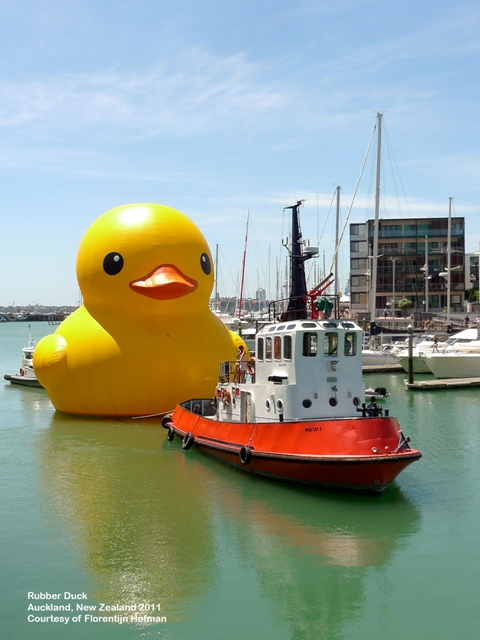
\includegraphics[width=0.95\textwidth]{img/rubberduck.jpg}
  \caption{caption}
  \label{fig:label}
\end{figure}





